%%%%%%%%%%%%%%%%%%%%%%%%%%%%%%%%%%%%%%%%%
% APA Assignment Article
% LaTeX Template
% Version 2.0 (February 7, 2023)
%
% This template originates from:
% https://www.LaTeXTemplates.com
%
% Author:
% Vel (vel@latextemplates.com)
%
% License:
% CC BY-NC-SA 4.0 (https://creativecommons.org/licenses/by-nc-sa/4.0/)
%
% NOTE: The bibliography needs to be compiled using the biber engine.
%
%%%%%%%%%%%%%%%%%%%%%%%%%%%%%%%%%%%%%%%%%

%----------------------------------------------------------------------------------------
%	PACKAGES AND OTHER DOCUMENT CONFIGURATIONS
%----------------------------------------------------------------------------------------

\documentclass[
	letterpaper, % Paper size, use either a4paper or letterpaper
	10pt, % Default font size, can also use 11pt or 12pt, although this is not recommended
	unnumberedsections, % Comment to enable section numbering
	twoside, % Two side traditional mode where headers and footers change between odd and even pages, comment this option to make them fixed
]{APAAssignment}

\addbibresource{bibliography.bib} % BibLaTeX bibliography file

\runninghead{MICS CYBER 252, Fall-2024 Written Assignment Unit 3} % A shortened article title to appear in the running head, leave this command empty for no running head

\footertext{\textit{Written Assignment Unit 3 (3.5.2)  } (MICS CYBER 252, Fall -2024)} % Text to appear in the footer, leave this command empty for no footer text

\setcounter{page}{1} % The page number of the first page, set this to a higher number if the article is to be part of an issue or larger work

%----------------------------------------------------------------------------------------
%	TITLE SECTION
%----------------------------------------------------------------------------------------

\usepackage[title,toc,titletoc]{appendix}
\usepackage{titlesec}
\usepackage{lscape}
\usepackage{fontawesome}

\title{Written Assignment Unit 3 \\ MICS-252, Fall 2024} % Article title, use manual lines breaks (\\) to beautify the layout

% Authors are listed in a comma-separated list with superscript numbers indicating affiliations
% \thanks{} is used for any text that should be placed in a footnote on the first page, such as the corresponding author's email, journal acceptance dates, a copyright/license notice, keywords, etc
% Affiliations are output in the \date{} command
\date{UC Berkleley School of Information \\
MICS Course 252 Fall 2024 (Kristy Westphal)
}


\author{
	Prepared by: Karl-Johan Westhoff \\
	email: \href{mailto:kjwesthoff@berkeley.edu}{kjwesthoff@berkeley.edu}
}


% % Full-width abstract
% \renewcommand{\maketitlehookd}{%
% 	\begin{abstract}
% 		\noindent Lorem ipsum dolor sit amet,rta porttitor.
% 	\end{abstract}
% }

%----------------------------------------------------------------------------------------

\setcounter{tocdepth}{5}
\setcounter{secnumdepth}{5}
\usepackage[title]{appendix}

\begin{document}
\onecolumn
\maketitle % Output the title section

%----------------------------------------------------------------------------------------
%	ARTICLE CONTENTS
%----------------------------------------------------------------------------------------

\section{Introduction}
For the first 2 weeks we have been working on web applications, I decided to continue on this topic for the SOC Tools, as discussed in class a SOC processes a firehose of information, and deploys fascinating tools\footnote{Security information and event management (SIEM)} and processes to do that. I wanted to look at some of the tools that collect and generate the data:

\begin{itemize}
	\item Web Application Firewalls (WAF), which apart from blocking stuff, 'of course' also logs its findings
	\item Intrusion Detection Systems (IDS), which monitors network traffic and reports suspicious activity 
\end{itemize}

\subsection{'Things' going to the cloud}
Cloud web applications are often distributed into "microservice" architectures where data is retrieved from APIs serving multiple applications rather than managed and retrieved directly from e.g. a dedicated database\footnote{I am myself 'guilty' of developing an application with more microservices than users at one point..}. 

The distributed-ness poses a new set of challenges for web security. The distributed architecture allows for a lot of different technologies to work together, often developed using "someone else's code" from open source libraries. Free Open Source Software (FOSS) is wonderful when you are a developer: you can usually find that someone has already solved the problem you are working on. But, there may be un-discovered vulnerabilities in the code, the risk needs to be mitigated somehow by:

\begin{itemize}
	\item Keeping inventory of the code and versions used (SBOM). 
	\item Deploy systems for detecting and preventing attacks (WAF and IDS).
\end{itemize}

With modern DevOps deployment where API's and services can be developed and deployed quickly. Security Operations (SecOps) needed to be adapted and security was shoehorned into the DevOps acronym, it is now referred to as DevSecOps\footnote{Shannon Lietz of Intuit is often credited with coining the term\cite{DevSecOps}}. The intention being that security is not to be regarded as an afterthought but part of the development cycles.  

With distributed applications there is a larger attack surface, there are more http endpoints that can be hit and the OWASP top 10 applies to all of them. The A01:2021-Broken Access control \cite{OWASPtop10} has probably moved to 1st. place in 2021 as Access and Identity control needs to be managed for all http endpoints in the distributed applications.       

\section{Web Application Firewalls}
WAF's protect web applications and covers many of the items in the OWASP top 10 list \cite{OWASPtop10}. WAF's scope is limited to the HTTP/S Protocol and WAF's are focused on analysis of http requests and responses. WAF's can be deployed in front of web applications or as part of other infrastructure e.g. reverse proxies and cloud load balancers.   

\subsection{WAF vs. "Ordinary" Firewall}
Firewalls in general works by allowing or blocking traffic on specific transport layer ports and ranges of IP addresses. Sometimes firewalls also work as 'stateful' where in and out going package ip's and ports are compared and grouped into sessions (i.e related traffic between the server and a client) and evaluated based on the relations between packets. More fancy firewalls also 'open' the packets and inspects parts of the packet payload, this requires more computing resources. 

I guess a WAF falls into the 'fancy firewall' category: HTTP/S traffic happens at the application layer of the OSI model and hence relates to the TCP/UDP packet payload. However, a difference to ordinary firewalls is that WAF's are specialized to work on http requests, since the traffic needs to be decrypted and parsed by the web server anyway, some the resource overhead from the WAF can be mitigated by doing some of the web servers work on the WAF while checking the traffic.    

\subsection{WAF in the cloud}
Much like with ordinary firewalls where one instance protects a whole subnet, WAF's can be deployed with a reverse proxy in front of a distributed web application, putting a WAF in front of the traffic can help mitigate some of the risk associated with FOSS and the complexity associated with distributed web apps.


\subsection{WAF examples}
As WAF's are based on analyzing the packet payloads and http query strings; 'it runs some code', checking if attacks are occurring e.g. by looking for:

\begin{itemize}
	\item 'special' characters for injection attacks
 	\item if passphrase spraying is being attempted
    \item etc. from the OWASP top 10
\end{itemize} 

For that, it needs to keep track of multiple packets to track sessions and TCP streams, many vendors advertize leveraging machine learning for this in their WAF's\cite{OpenappsecWaf}.

\subsubsection{Types of WAF's:} WAF's are deployed in different settings depending on how the web applications they protect are deployed, in all cases WAF's need adequate processing power and network bandwidth.
\begin{itemize}
	\item{\textbf{Host Based}: On the same physical hardware and OS as the web application}
	\item{\textbf{Network Based}: On a separate 'box' on the network, for example with a reverse proxy}
	\item{\textbf{Cloud Based}: As part of the cloud provider's monitoring and logging systems, usually provided as a paid-for service\footnote{['\textit{Your Acronym Here}']aaS} by the cloud provider} 
\end{itemize}


\subsubsection{WAF software providers:}
Most modern web applications are cloud deployed, A list of ten popular WAF's is presented in \cite{OpenappsecWaf}, some examples are: 

\begin{itemize}
	
	\item{\textbf{Cloud vendor based}: Provided as a service where you host you web application: 
	\begin{itemize}
		\item "Azure WAFv2 \cite{AzureWAF}"
		\item "AWS WAF \cite{AWSWAF}"
	\end{itemize}
	}
	
	\item{\textbf{Security providers}: Managed solutions for outsourcing the concern:
	\begin{itemize}
		\item "Cloudflare WAF \cite{CloudflareWAF}"
		\item "AppTrana Manage WAF \cite{AppTrana-WAF}"
	\end{itemize}
	}
	
	\item{
		\textbf{Open Source}: For research and budget oriented companies e.g. NGO's, requires some in-house security expertise: 
		\begin{itemize}
			\item "open-appsec \cite{open-appsec}"
			\item "OWASP Corza \cite{OWASPcorsa}"
		\end{itemize}
	} 
\end{itemize}


\section{Intrusion Detection Systems}
Intrusion detection systems (IDS) monitor network traffic and reports/alerts if it recognizes suspicious activity, sometimes IDS also actively blocks traffic, then referred to as an Intrusion Prevention System (IPS). IDS systems often deliver data to a SIEM for further analysis. IDS's can be deployed both on individual hosts or at strategic places in networks, for example on a switch's promiscuous/mirror port analyzing all network traffic going through the switch. Just like WAF's IDS's need to analyze network packets, a key difference is that IDS's are not limited to HTTP/S traffic, but they are scoped to the full spread of protocols running on the transport layer.

IDS's usually work by applying rules to simple packet analysis in individual transport layer packets, checking for source/destination IP's, ports and which protocols are transmitted (much like a firewall). IDS also keep track of series of packets and their relations in sessions (stateful protocol analysis). Furthermore, most IDS's also look at anomalies in traffic, many vendors advertise deploying machine learning here. IDS can detect more advanced attacks, one example is the 'EternalBlue' attack on Microsoft's SMB protocol, the attack was detectable by looking at a specific pattern of TCP traffic on port 446, and quickly distributing IDS rules helped mitigate the attack (See Snort Rule example in Appendix \ref{app:SnortEternalBlue}). 

IDS applies predefined rules often based on known patterns for malicious traffic (signatures) to trigger alerts. IDS rules need to be maintained and updated to reflect the threats on the internet.    

\subsection{IDS in the cloud}
Network traffic in cloud is virtualized and you cannot just plug an IDS into a mirror port on a switch to monitor the network, you are somewhat reliant on the cloud provider to deliver data for monitoring. IDS could be deployed on every cloud instance but that would create a large workload, both of extra compute resources on each instance, and a high workload for maintaining and deploying signatures to many instances.       

\subsubsection{Case study: Snort on Oracle Cloud}
For the MICS Cyber210 networking class we wanted to build an "Attack and Defend" lab with a monitored network containing vulnerable hosts, and detect attacks on these using Snort\cite{SNORT}. Instead of actually using hardware we decided to build a virtual lab using Oracle Cloud\footnote{The intention was to deploy deliberately
vulnerable infrastructure to test, not all cloud providers make this easy. We found that Oracle Cloud has a 30day/300\$ trial period which we decided to burn on the project.}. It turned out it wasn't so easy to rig a cloud network with host based software. Apart from separating the network to hide the vulnerable machines from the internet (obviously). We wanted to monitor traffic on a subnet, to simulate the promiscuous/mirror port on a fictive switch, we had to route the traffic from the vulnerable machines to the IDS using a load balancer and virtual tap's (VTAP) on each of the instances we wanted to monitor to a Ubuntu instance running Snort see Figure \ref{fig:AttackAndDefendLab} 

\begin{figure}[!htp] % Single column figure
	\centering
	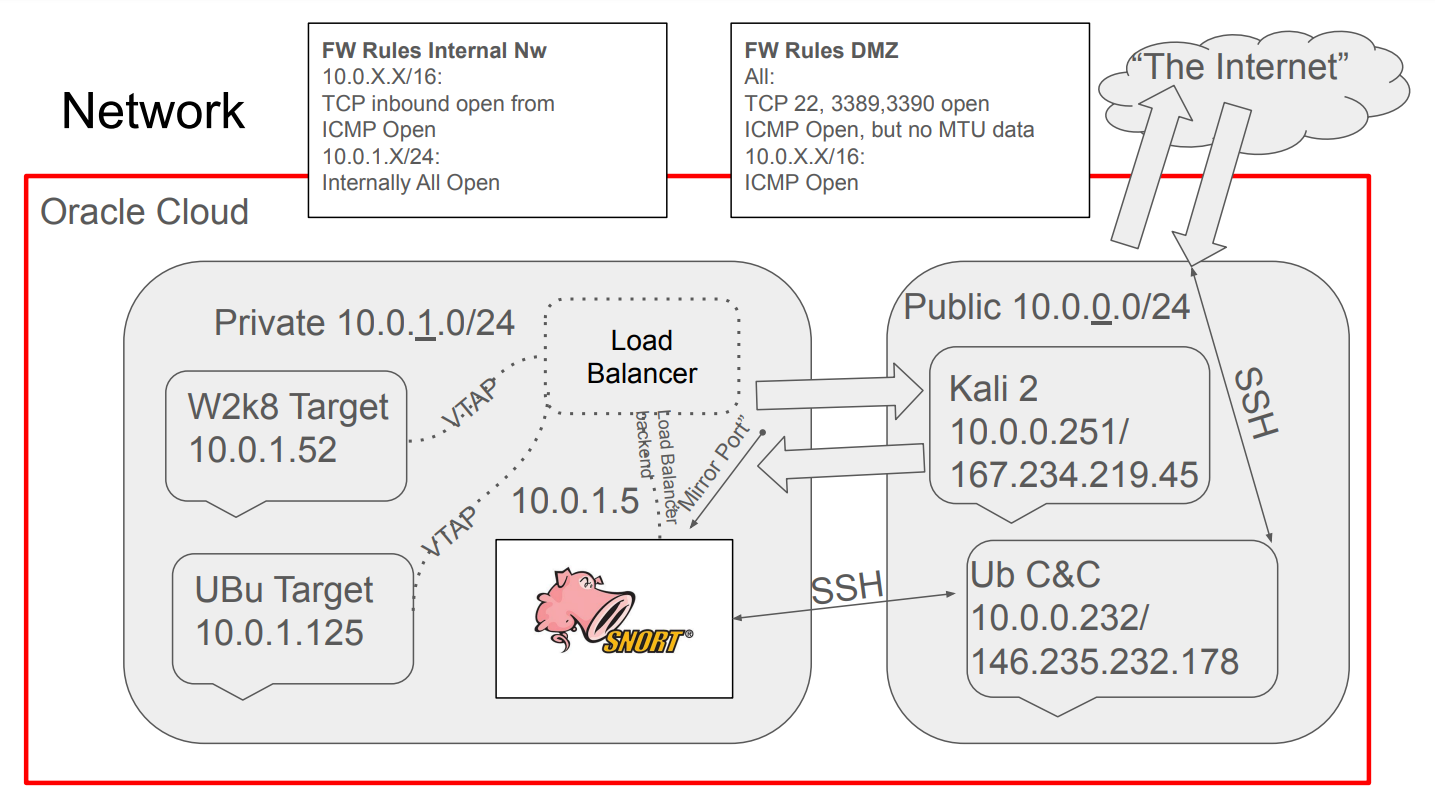
\includegraphics[width=\linewidth]{AttackAndDefendLab.png}
	\caption{Attack and Defend Lab Diagram, for a project for Cyber210. The idea is that attacks are performed on the targets from the Kali instance (attacker logged in via RDP), and detected by defenders (subscribing to Snort alerts via SSH). The dotted lines indicate the traffic workarounds simulating a physical mirrored port on a switch using VTAPs and a load balancer.}
	\label{fig:AttackAndDefendLab}
\end{figure}

\subsection{IDS Examples}


There seems to be  some consensus that IDS's/IPS can be split into 2 categories:

\begin{itemize}
	\item \textbf{Host-based Intrusion Detection System (HIDS)}: 
	\begin{itemize}
		\item Installed on every host, may trace network activity to a specific application on that host.
		\item Uses resources from the host and needs to be maintained and signatures updated on that host.
	\end{itemize}
	\item \textbf{Network Intrusion Detection System (NIDS)}: 
	\begin{itemize}
		\item Monitors a whole subnet using one instance (less to maintain) 
		\item Needs to keep up with the traffic (may be a challenge on large networks)
	\end{itemize}
\end{itemize}

Beyond \textbf{'H'} and \textbf{'N'} IDS, sources and vendors seem to come up with a variety of definitions:

\begin{itemize}
	\item Wireless Intrusion Prevention System (WIPS):   Monitors Wi-Fi networks \cite{FortinetIPSdefinitiopns}
	\item Network Behavior Analysis (NBA): Detect what might be associated with distributed denial of service (DDoS) attacks \cite{FortinetIPSdefinitiopns}
	\item Network Node Intrusion Detection System (NNIDS): Watches over each node connected to your network \cite{HelixstormIDSdefinitiopns}.
	\item Protocol-Based Intrusion Detection System (PIDS): Analyzes the HTTP or HTTPS protocol stream between your devices and the server\cite{HelixstormIDSdefinitiopns}.
	\item Etc. Put in your own use case with associated acronym here..
\end{itemize}

Some examples of IDS/IPS systems are shown in Table \ref{tab:IPSProdicts}:

\begin{table}[!ht]
    \centering
    \begin{tabular}{|p{2.2cm}|p{1.5cm}|p{1.5cm}|p{1.5cm}|p{1.5cm}|p{1.5cm}|p{1.5cm}|p{1.5cm}|}
    \hline
        \textbf{Features/IDS} & \textbf{Real-time Monitoring} & \textbf{Log Management} & \textbf{Signature-based Detection} & \textbf{Anomaly-based Detection} & \textbf{Open Source} & \textbf{Cloud Integration} & \textbf{Free Version Available} \\ \hline
        \textbf{ManageEngine EventLog Analyzer} & Yes & Yes & Yes & Yes & No & Yes & No \\ \hline
        \textbf{ManageEngine Log360} & Yes & Yes & Yes & Yes & No & Yes & No \\ \hline
        \textbf{ESET Protect} & Yes & Yes & Yes & Yes & No & Yes & No \\ \hline
        \textbf{Snort} & Yes & Yes & Yes & Yes & Yes & No & Yes \\ \hline
        \textbf{SolarWinds Security Event Manager} & Yes & Yes & Yes & Yes & No & Yes & No \\ \hline
        \textbf{OSSEC} & Yes & Yes & Yes & Yes & Yes & No & Yes \\ \hline
        \textbf{Gatewatcher AIonIQ} & Yes & Yes & Yes & Yes & No & Yes & No \\ \hline
        \textbf{CrowdSec} & Yes & Yes & Yes & Yes & Yes & Yes & Yes \\ \hline
        \textbf{Suricata} & Yes & Yes & Yes & Yes & Yes & No & Yes \\ \hline
        \textbf{Zeek} & Yes & Yes & Yes & Yes & Yes & No & Yes \\ \hline
        \textbf{Security Onion} & Yes & Yes & Yes & Yes & Yes & No & Yes \\ \hline
        \textbf{AIDE} & Yes & No & No & Yes & Yes & No & Yes \\ \hline
    \end{tabular}
	\caption{Comparison of different IDS/IPS products, data from \cite{ComparitechIPSComparison}} 
	\label{tab:IPSProdicts}
\end{table}


\section{Conclusion}
Web Application Firewalls (WAF) and Intrusion Detection Systems (IDS) are important sources of data to the security operation. IDS's and WAF's can help mitigate some of the risk associated with moving infrastructure and company functions to cloud based web applications. With applications being deployed on 'someone else's computer' often using 'someone else's code', it is however important to monitor the traffic and protect the applications. By limiting data infrastructure to use  HTTP/S traffic, the attack surface actually gets smaller and tools can be simplified and made more efficient (WAF is an example hereof). Most services could be made web based, managers and most enterprise support functions do not need computers with advanced OS systems, but could do all work on devices with a web browser only. The security can then be shifted more towards Identity and Access Management (IAM) and a focus on social engineering attacks.


%----------------------------------------------------------------------------------------
%	 REFERENCES
%----------------------------------------------------------------------------------------
\clearpage
\printbibliography % Output the bibliography

%----------------------------------------------------------------------------------------



%----------------------------------------------------------------------------------------
%	 Appendices
%----------------------------------------------------------------------------------------

\appendix


\clearpage
\chapter{Appendices}
\begin{appendices}
\section{SNORT rule for "EternalBlue", SID 41978 see\cite{SnortEternalBlue}}\label{app:SnortEternalBlue}

\begin{lstlisting}
	alert tcp $EXTERNAL_NET any -> $HOME_NET 445 (msg:"OS-WINDOWS Microsoft Windows SMB remote code execution attempt"; flow:to_server,established; content:"|FF|SMB3|00 00 00 00|"; depth:9; offset:4; byte_extract:2,26,TotalDataCount,relative,little; byte_test:2,>,TotalDataCount,20,relative,little; metadata:policy balanced-ips drop, policy connectivity-ips drop, policy security-ips drop, ruleset community, service netbios-ssn; reference:cve,2017-0144; reference:cve,2017-0146; reference:url,isc.sans.edu/forums/diary/ETERNALBLUE+Possible+Window+SMB+Buffer+Overflow+0Day/22304/; reference:url,technet.microsoft.com/en-us/security/bulletin/MS17-010; classtype:attempted-admin; sid:41978; rev:3;)
\end{lstlisting}

I had ChatGPT write out following explanation to the rule, see Figure \ref{fig:SnortExaplin}

\begin{figure}[!htp] % Single column figure
	\centering
	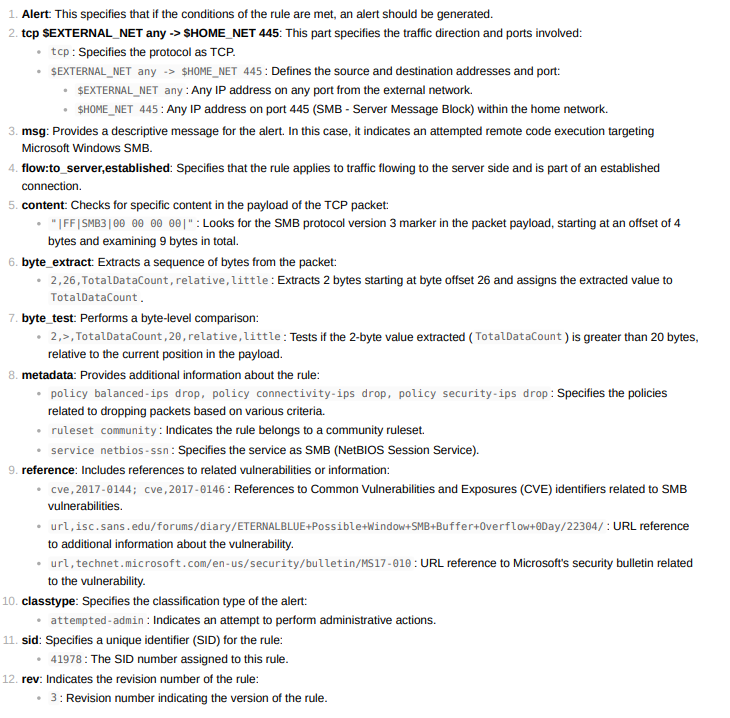
\includegraphics[width=\linewidth]{ChatGPTExplanation.png}
	\caption{Explanation for the  SID 41978 snort Rule, generated using ChatGPT }
	\label{fig:SnortExaplin}
\end{figure}

%\hypertarget{webgoat-setup}{%


% \begin{figure}[!ht] % Single column figure
% 	\centering
% 	\includegraphics[width=\linewidth]{IdentAndAuthBypass.png}
% 	\caption{Authentication reset bypassed by changing the secQuestion names the POST request payload}
% 	\label{fig:app:AuthBypass}
% \end{figure}


\end{appendices}
\end{document}
